\documentclass[twoside]{book}

% Packages required by doxygen
\usepackage{fixltx2e}
\usepackage{calc}
\usepackage{doxygen}
\usepackage[export]{adjustbox} % also loads graphicx
\usepackage{graphicx}
\usepackage[utf8]{inputenc}
\usepackage{makeidx}
\usepackage{multicol}
\usepackage{multirow}
\PassOptionsToPackage{warn}{textcomp}
\usepackage{textcomp}
\usepackage[nointegrals]{wasysym}
\usepackage[table]{xcolor}

% Font selection
\usepackage[T1]{fontenc}
\usepackage[scaled=.90]{helvet}
\usepackage{courier}
\usepackage{amssymb}
\usepackage{sectsty}
\renewcommand{\familydefault}{\sfdefault}
\allsectionsfont{%
  \fontseries{bc}\selectfont%
  \color{darkgray}%
}
\renewcommand{\DoxyLabelFont}{%
  \fontseries{bc}\selectfont%
  \color{darkgray}%
}
\newcommand{\+}{\discretionary{\mbox{\scriptsize$\hookleftarrow$}}{}{}}

% Page & text layout
\usepackage{geometry}
\geometry{%
  a4paper,%
  top=2.5cm,%
  bottom=2.5cm,%
  left=2.5cm,%
  right=2.5cm%
}
\tolerance=750
\hfuzz=15pt
\hbadness=750
\setlength{\emergencystretch}{15pt}
\setlength{\parindent}{0cm}
\setlength{\parskip}{3ex plus 2ex minus 2ex}
\makeatletter
\renewcommand{\paragraph}{%
  \@startsection{paragraph}{4}{0ex}{-1.0ex}{1.0ex}{%
    \normalfont\normalsize\bfseries\SS@parafont%
  }%
}
\renewcommand{\subparagraph}{%
  \@startsection{subparagraph}{5}{0ex}{-1.0ex}{1.0ex}{%
    \normalfont\normalsize\bfseries\SS@subparafont%
  }%
}
\makeatother

% Headers & footers
\usepackage{fancyhdr}
\pagestyle{fancyplain}
\fancyhead[LE]{\fancyplain{}{\bfseries\thepage}}
\fancyhead[CE]{\fancyplain{}{}}
\fancyhead[RE]{\fancyplain{}{\bfseries\leftmark}}
\fancyhead[LO]{\fancyplain{}{\bfseries\rightmark}}
\fancyhead[CO]{\fancyplain{}{}}
\fancyhead[RO]{\fancyplain{}{\bfseries\thepage}}
\fancyfoot[LE]{\fancyplain{}{}}
\fancyfoot[CE]{\fancyplain{}{}}
\fancyfoot[RE]{\fancyplain{}{\bfseries\scriptsize Generated by Doxygen }}
\fancyfoot[LO]{\fancyplain{}{\bfseries\scriptsize Generated by Doxygen }}
\fancyfoot[CO]{\fancyplain{}{}}
\fancyfoot[RO]{\fancyplain{}{}}
\renewcommand{\footrulewidth}{0.4pt}
\renewcommand{\chaptermark}[1]{%
  \markboth{#1}{}%
}
\renewcommand{\sectionmark}[1]{%
  \markright{\thesection\ #1}%
}

% Indices & bibliography
\usepackage{natbib}
\usepackage[titles]{tocloft}
\setcounter{tocdepth}{3}
\setcounter{secnumdepth}{5}
\makeindex

% Hyperlinks (required, but should be loaded last)
\usepackage{ifpdf}
\ifpdf
  \usepackage[pdftex,pagebackref=true]{hyperref}
\else
  \usepackage[ps2pdf,pagebackref=true]{hyperref}
\fi
\hypersetup{%
  colorlinks=true,%
  linkcolor=blue,%
  citecolor=blue,%
  unicode%
}

% Custom commands
\newcommand{\clearemptydoublepage}{%
  \newpage{\pagestyle{empty}\cleardoublepage}%
}

\usepackage{caption}
\captionsetup{labelsep=space,justification=centering,font={bf},singlelinecheck=off,skip=4pt,position=top}

%===== C O N T E N T S =====

\begin{document}

% Titlepage & ToC
\hypersetup{pageanchor=false,
             bookmarksnumbered=true,
             pdfencoding=unicode
            }
\pagenumbering{alph}
\begin{titlepage}
\vspace*{7cm}
\begin{center}%
{\Large My Project }\\
\vspace*{1cm}
{\large Generated by Doxygen 1.8.12}\\
\end{center}
\end{titlepage}
\clearemptydoublepage
\pagenumbering{roman}
\tableofcontents
\clearemptydoublepage
\pagenumbering{arabic}
\hypersetup{pageanchor=true}

%--- Begin generated contents ---
\chapter{Hierarchical Index}
\section{Class Hierarchy}
This inheritance list is sorted roughly, but not completely, alphabetically\+:\begin{DoxyCompactList}
\item \contentsline{section}{File}{\pageref{class_file}}{}
\item \contentsline{section}{Filesystem}{\pageref{class_filesystem}}{}
\item \contentsline{section}{Focusable}{\pageref{class_focusable}}{}
\item \contentsline{section}{Game}{\pageref{class_game}}{}
\item \contentsline{section}{Game\+Listener}{\pageref{class_game_listener}}{}
\begin{DoxyCompactList}
\item \contentsline{section}{Window}{\pageref{class_window}}{}
\begin{DoxyCompactList}
\item \contentsline{section}{Dock}{\pageref{class_dock}}{}
\item \contentsline{section}{Terminal\+Window}{\pageref{class_terminal_window}}{}
\end{DoxyCompactList}
\end{DoxyCompactList}
\item \contentsline{section}{Graphics}{\pageref{class_graphics}}{}
\item \contentsline{section}{Input}{\pageref{class_input}}{}
\item \contentsline{section}{Sprite}{\pageref{class_sprite}}{}
\end{DoxyCompactList}

\chapter{Class Index}
\section{Class List}
Here are the classes, structs, unions and interfaces with brief descriptions\+:\begin{DoxyCompactList}
\item\contentsline{section}{\hyperlink{class_dock}{Dock} }{\pageref{class_dock}}{}
\item\contentsline{section}{\hyperlink{class_file}{File} }{\pageref{class_file}}{}
\item\contentsline{section}{\hyperlink{class_filesystem}{Filesystem} }{\pageref{class_filesystem}}{}
\item\contentsline{section}{\hyperlink{class_focusable}{Focusable} }{\pageref{class_focusable}}{}
\item\contentsline{section}{\hyperlink{class_game}{Game} }{\pageref{class_game}}{}
\item\contentsline{section}{\hyperlink{class_game_listener}{Game\+Listener} }{\pageref{class_game_listener}}{}
\item\contentsline{section}{\hyperlink{class_graphics}{Graphics} }{\pageref{class_graphics}}{}
\item\contentsline{section}{\hyperlink{class_input}{Input} }{\pageref{class_input}}{}
\item\contentsline{section}{\hyperlink{class_sprite}{Sprite} }{\pageref{class_sprite}}{}
\item\contentsline{section}{\hyperlink{class_terminal_window}{Terminal\+Window} }{\pageref{class_terminal_window}}{}
\item\contentsline{section}{\hyperlink{class_window}{Window} }{\pageref{class_window}}{}
\end{DoxyCompactList}

\chapter{Class Documentation}
\hypertarget{class_dock}{}\section{Dock Class Reference}
\label{class_dock}\index{Dock@{Dock}}


Inheritance diagram for Dock\+:\nopagebreak
\begin{figure}[H]
\begin{center}
\leavevmode
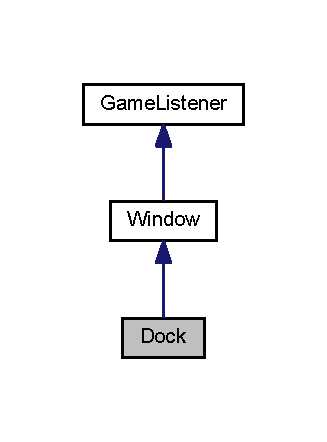
\includegraphics[width=157pt]{class_dock__inherit__graph}
\end{center}
\end{figure}


Collaboration diagram for Dock\+:\nopagebreak
\begin{figure}[H]
\begin{center}
\leavevmode
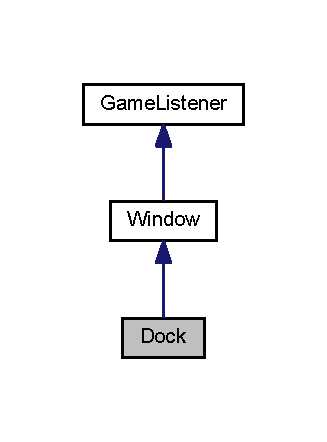
\includegraphics[width=157pt]{class_dock__coll__graph}
\end{center}
\end{figure}
\subsection*{Public Member Functions}
\begin{DoxyCompactItemize}
\item 
\hypertarget{class_dock_ab6358124b92d41bee01b47aae633ba4e}{}\label{class_dock_ab6358124b92d41bee01b47aae633ba4e} 
{\bfseries Dock} (\hyperlink{class_game}{Game} $\ast$g, int x, int y, int w, int h)
\item 
\hypertarget{class_dock_a4dc4c069680a6fb3bb6e8656296a8bb7}{}\label{class_dock_a4dc4c069680a6fb3bb6e8656296a8bb7} 
void {\bfseries move} (int x, int y) override
\item 
\hypertarget{class_dock_a2e64fed55b6e670af42f4b360f2210ea}{}\label{class_dock_a2e64fed55b6e670af42f4b360f2210ea} 
void {\bfseries draw} (\hyperlink{class_graphics}{Graphics} \&g) override
\item 
\hypertarget{class_dock_a9ff981e9c2dfe3614e332aa4c4f8fcee}{}\label{class_dock_a9ff981e9c2dfe3614e332aa4c4f8fcee} 
void {\bfseries on\+Mouse} (bool b, int x, int y) override
\end{DoxyCompactItemize}
\subsection*{Additional Inherited Members}


The documentation for this class was generated from the following files\+:\begin{DoxyCompactItemize}
\item 
headers/Dock.\+h\item 
src/Dock.\+cpp\end{DoxyCompactItemize}

\hypertarget{class_file}{}\section{File Class Reference}
\label{class_file}\index{File@{File}}
\subsection*{Public Member Functions}
\begin{DoxyCompactItemize}
\item 
\hypertarget{class_file_a69d092c3f2d97377d5b62447b8cbf884}{}\label{class_file_a69d092c3f2d97377d5b62447b8cbf884} 
{\bfseries File} (\hyperlink{class_filesystem}{Filesystem} $\ast$f, const std\+::string \&name)
\item 
\hypertarget{class_file_a209295d716a644c786a8766922f59905}{}\label{class_file_a209295d716a644c786a8766922f59905} 
{\bfseries File} (\hyperlink{class_filesystem}{Filesystem} $\ast$f, const std\+::string \&name, const std\+::string \&cat)
\item 
\hypertarget{class_file_aa041ad660c8322eecb72333a80bd1c48}{}\label{class_file_aa041ad660c8322eecb72333a80bd1c48} 
std\+::string {\bfseries cat} ()
\item 
\hypertarget{class_file_a479b1c28c7ad57ccf1e76b8305221a64}{}\label{class_file_a479b1c28c7ad57ccf1e76b8305221a64} 
virtual void {\bfseries run} (\hyperlink{class_terminal_window}{Terminal\+Window} $\ast$t)
\end{DoxyCompactItemize}
\subsection*{Public Attributes}
\begin{DoxyCompactItemize}
\item 
\hypertarget{class_file_a94e032201b6182d92d0eadbea43182ac}{}\label{class_file_a94e032201b6182d92d0eadbea43182ac} 
std\+::string {\bfseries \+\_\+name}
\end{DoxyCompactItemize}


The documentation for this class was generated from the following files\+:\begin{DoxyCompactItemize}
\item 
headers/File.\+h\item 
src/File.\+cpp\end{DoxyCompactItemize}

\hypertarget{class_filesystem}{}\section{Filesystem Class Reference}
\label{class_filesystem}\index{Filesystem@{Filesystem}}
\subsection*{Public Member Functions}
\begin{DoxyCompactItemize}
\item 
\hypertarget{class_filesystem_add49abb4ab07ed5e30cecf13a4788763}{}\label{class_filesystem_add49abb4ab07ed5e30cecf13a4788763} 
{\bfseries Filesystem} (const std\+::string \&name)
\item 
\hypertarget{class_filesystem_aca3f43e7007db68ee3d8c7aa54817d50}{}\label{class_filesystem_aca3f43e7007db68ee3d8c7aa54817d50} 
void {\bfseries add\+Folder} (const std\+::string \&s)
\item 
\hypertarget{class_filesystem_a4077af11b72a6b4a799e8df3536cc915}{}\label{class_filesystem_a4077af11b72a6b4a799e8df3536cc915} 
void {\bfseries add\+File} (\hyperlink{class_file}{File} $\ast$f)
\item 
\hypertarget{class_filesystem_a99756d50bf21030eccdc02f20bfac839}{}\label{class_filesystem_a99756d50bf21030eccdc02f20bfac839} 
std\+::string {\bfseries get\+Cwd} ()
\item 
\hypertarget{class_filesystem_acde9704dcfc564002841cd3c7a97e439}{}\label{class_filesystem_acde9704dcfc564002841cd3c7a97e439} 
std\+::string {\bfseries cd} (const std\+::string \&dir)
\item 
\hypertarget{class_filesystem_a57bb81a4d8a2f2d1fec16c60399d6820}{}\label{class_filesystem_a57bb81a4d8a2f2d1fec16c60399d6820} 
std\+::vector$<$ std\+::string $>$ {\bfseries ls} (const std\+::string \&s)
\item 
\hypertarget{class_filesystem_ad07ad4eca174dc1ce88df4050dadd4cf}{}\label{class_filesystem_ad07ad4eca174dc1ce88df4050dadd4cf} 
std\+::string {\bfseries cat} (const std\+::string \&file)
\item 
\hypertarget{class_filesystem_adb6294ff510eab4f4e704dd0d1dcd247}{}\label{class_filesystem_adb6294ff510eab4f4e704dd0d1dcd247} 
std\+::string {\bfseries to\+Root} (const std\+::string \&path)
\item 
\hypertarget{class_filesystem_ae6ccb1af9245376cc2eedfe0e6fc38d4}{}\label{class_filesystem_ae6ccb1af9245376cc2eedfe0e6fc38d4} 
void {\bfseries run} (const std\+::string \&file)
\end{DoxyCompactItemize}
\subsection*{Static Public Member Functions}
\begin{DoxyCompactItemize}
\item 
\hypertarget{class_filesystem_a225c02ba382d5bd91bc1cb0180d12ef7}{}\label{class_filesystem_a225c02ba382d5bd91bc1cb0180d12ef7} 
static \hyperlink{class_filesystem}{Filesystem} $\ast$ {\bfseries create\+Filesystem} (const std\+::string \&name)
\end{DoxyCompactItemize}


The documentation for this class was generated from the following files\+:\begin{DoxyCompactItemize}
\item 
headers/Filesystem.\+h\item 
src/Filesystem.\+cpp\end{DoxyCompactItemize}

\hypertarget{class_focusable}{}\section{Focusable Class Reference}
\label{class_focusable}\index{Focusable@{Focusable}}
\subsection*{Public Member Functions}
\begin{DoxyCompactItemize}
\item 
\hypertarget{class_focusable_aac64d80112af583baf9ea8454ed8c26a}{}\label{class_focusable_aac64d80112af583baf9ea8454ed8c26a} 
virtual void {\bfseries render} (\hyperlink{class_graphics}{Graphics} $\ast$g)
\item 
\hypertarget{class_focusable_abedddc31795aa7df783ada9eb81b5138}{}\label{class_focusable_abedddc31795aa7df783ada9eb81b5138} 
bool {\bfseries focus} ()
\item 
\hypertarget{class_focusable_a2a33756c950740cb2c7597479df5727d}{}\label{class_focusable_a2a33756c950740cb2c7597479df5727d} 
bool {\bfseries unfocus} ()
\end{DoxyCompactItemize}


The documentation for this class was generated from the following file\+:\begin{DoxyCompactItemize}
\item 
headers/Focusable.\+h\end{DoxyCompactItemize}

\hypertarget{class_game}{}\section{Game Class Reference}
\label{class_game}\index{Game@{Game}}


Collaboration diagram for Game\+:\nopagebreak
\begin{figure}[H]
\begin{center}
\leavevmode
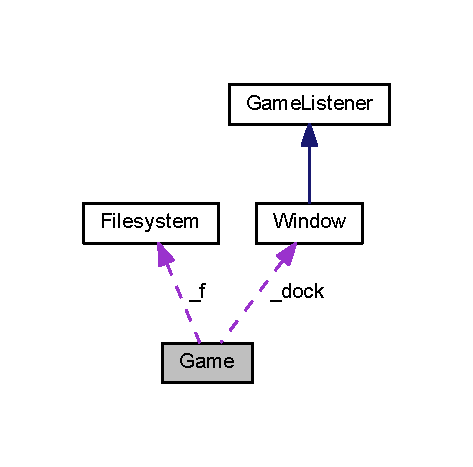
\includegraphics[width=227pt]{class_game__coll__graph}
\end{center}
\end{figure}
\subsection*{Public Member Functions}
\begin{DoxyCompactItemize}
\item 
\hypertarget{class_game_a50cc765d80923a84ffc1f27eb6f3131b}{}\label{class_game_a50cc765d80923a84ffc1f27eb6f3131b} 
\hyperlink{class_window}{Window} $\ast$ {\bfseries get\+Window} (int i)
\item 
\hypertarget{class_game_a239067e33c0bc2a13556835a3b256d97}{}\label{class_game_a239067e33c0bc2a13556835a3b256d97} 
void {\bfseries focus\+Window} (int pos)
\item 
\hypertarget{class_game_a95b3e1391bebb6e364eba411cc9dbe17}{}\label{class_game_a95b3e1391bebb6e364eba411cc9dbe17} 
int {\bfseries get\+Window\+At\+Location} (int x, int y)
\item 
\hypertarget{class_game_a887a40c61bff9edff550bdd26cc96448}{}\label{class_game_a887a40c61bff9edff550bdd26cc96448} 
void {\bfseries add\+Window} (\hyperlink{class_window}{Window} $\ast$w)
\item 
\hypertarget{class_game_ad41f2e79cf1b47b8bbf8837c7757fcce}{}\label{class_game_ad41f2e79cf1b47b8bbf8837c7757fcce} 
void {\bfseries login} (const std\+::string \&user)
\item 
\hypertarget{class_game_a8dbcab05b5640a882abf5bc2038462ca}{}\label{class_game_a8dbcab05b5640a882abf5bc2038462ca} 
void {\bfseries add\+Game\+Listener} (\hyperlink{class_game_listener}{Game\+Listener} $\ast$g)
\end{DoxyCompactItemize}
\subsection*{Public Attributes}
\begin{DoxyCompactItemize}
\item 
\hypertarget{class_game_ade70038b3153f5f293636d6d56f94562}{}\label{class_game_ade70038b3153f5f293636d6d56f94562} 
std\+::vector$<$ \hyperlink{class_window}{Window} $\ast$ $>$ {\bfseries \+\_\+windows}
\item 
\hypertarget{class_game_a95f4c70882199f901d2bdb5246c07cd6}{}\label{class_game_a95f4c70882199f901d2bdb5246c07cd6} 
\hyperlink{class_window}{Window} $\ast$ {\bfseries \+\_\+dock}
\item 
\hypertarget{class_game_ab7c57ed53d2f36d767f917d0e216348f}{}\label{class_game_ab7c57ed53d2f36d767f917d0e216348f} 
\hyperlink{class_filesystem}{Filesystem} $\ast$ {\bfseries \+\_\+f}
\end{DoxyCompactItemize}


The documentation for this class was generated from the following files\+:\begin{DoxyCompactItemize}
\item 
headers/Game.\+h\item 
src/Game.\+cpp\end{DoxyCompactItemize}

\hypertarget{class_game_listener}{}\section{Game\+Listener Class Reference}
\label{class_game_listener}\index{Game\+Listener@{Game\+Listener}}


Inheritance diagram for Game\+Listener\+:\nopagebreak
\begin{figure}[H]
\begin{center}
\leavevmode
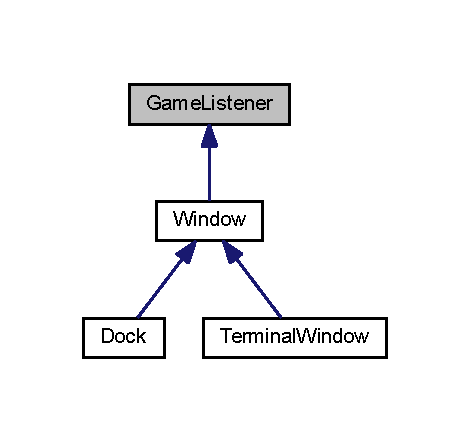
\includegraphics[width=226pt]{class_game_listener__inherit__graph}
\end{center}
\end{figure}
\subsection*{Public Member Functions}
\begin{DoxyCompactItemize}
\item 
\hypertarget{class_game_listener_a567361920fc494b68fda9d08b3222e1b}{}\label{class_game_listener_a567361920fc494b68fda9d08b3222e1b} 
void {\bfseries on\+Filesystem\+Change} (\hyperlink{class_filesystem}{Filesystem} $\ast$f)
\end{DoxyCompactItemize}


The documentation for this class was generated from the following file\+:\begin{DoxyCompactItemize}
\item 
headers/Game\+Listener.\+h\end{DoxyCompactItemize}

\hypertarget{class_graphics}{}\section{Graphics Class Reference}
\label{class_graphics}\index{Graphics@{Graphics}}
\subsection*{Public Member Functions}
\begin{DoxyCompactItemize}
\item 
\hypertarget{class_graphics_ac8578764cb1ae151e8e2294917c67128}{}\label{class_graphics_ac8578764cb1ae151e8e2294917c67128} 
S\+D\+L\+\_\+\+Surface $\ast$ {\bfseries load\+Image} (const std\+::string \&file\+Path)
\item 
\hypertarget{class_graphics_ac20be05864dabab875373957544cd6f1}{}\label{class_graphics_ac20be05864dabab875373957544cd6f1} 
void {\bfseries blit\+Surface} (S\+D\+L\+\_\+\+Texture $\ast$img, S\+D\+L\+\_\+\+Rect $\ast$src, S\+D\+L\+\_\+\+Rect $\ast$dest)
\item 
\hypertarget{class_graphics_a3ac4cb173d4661243afe6cff2c9ea0f5}{}\label{class_graphics_a3ac4cb173d4661243afe6cff2c9ea0f5} 
void {\bfseries draw\+Text} (const std\+::string \&text, int x, int y)
\item 
\hypertarget{class_graphics_a2cb7ca43cf024733c813a05240b2157c}{}\label{class_graphics_a2cb7ca43cf024733c813a05240b2157c} 
void {\bfseries set\+Font} (const std\+::string \&font, int size)
\item 
\hypertarget{class_graphics_adee5e3a62f8b9875b0816bed7bc327e5}{}\label{class_graphics_adee5e3a62f8b9875b0816bed7bc327e5} 
void {\bfseries set\+Color} (Uint8 r, Uint8 g, Uint8 b)
\item 
\hypertarget{class_graphics_abce690dc817c4c3648b0a56598acb3a8}{}\label{class_graphics_abce690dc817c4c3648b0a56598acb3a8} 
void {\bfseries set\+Color} (Uint8 r, Uint8 g, Uint8 b, Uint8 a)
\item 
\hypertarget{class_graphics_a8726be9cb0342c5492ff6adbd4bc81fa}{}\label{class_graphics_a8726be9cb0342c5492ff6adbd4bc81fa} 
void {\bfseries flip} ()
\item 
\hypertarget{class_graphics_a5006edbbdc540af376d4787f9d56fbdd}{}\label{class_graphics_a5006edbbdc540af376d4787f9d56fbdd} 
void {\bfseries clear} ()
\item 
\hypertarget{class_graphics_a490f6efb89fe1849ef8bde599e5d647c}{}\label{class_graphics_a490f6efb89fe1849ef8bde599e5d647c} 
void {\bfseries draw\+Line} (int x1, int y1, int x2, int y2)
\item 
\hypertarget{class_graphics_a74068ed7014bd8c965a71d8e1f9df9ca}{}\label{class_graphics_a74068ed7014bd8c965a71d8e1f9df9ca} 
void {\bfseries draw\+Rect} (int x1, int y1, int w, int h)
\item 
\hypertarget{class_graphics_ae874aa5745030706ca3813051280fe52}{}\label{class_graphics_ae874aa5745030706ca3813051280fe52} 
void {\bfseries fill\+Rect} (int x1, int y1, int w, int h)
\item 
\hypertarget{class_graphics_ab4399392db97b56a59a57bc357f1de48}{}\label{class_graphics_ab4399392db97b56a59a57bc357f1de48} 
S\+D\+L\+\_\+\+Renderer $\ast$ {\bfseries get\+Renderer} () const
\end{DoxyCompactItemize}


The documentation for this class was generated from the following files\+:\begin{DoxyCompactItemize}
\item 
headers/Graphics.\+h\item 
src/Graphics.\+cpp\end{DoxyCompactItemize}

\hypertarget{class_input}{}\section{Input Class Reference}
\label{class_input}\index{Input@{Input}}
\subsection*{Public Member Functions}
\begin{DoxyCompactItemize}
\item 
\hypertarget{class_input_a70f98f66cf753329e4dd186ead94c5dd}{}\label{class_input_a70f98f66cf753329e4dd186ead94c5dd} 
{\bfseries Input} (\hyperlink{class_game}{Game} $\ast$g)
\item 
\hypertarget{class_input_aa46ab29d639305a50c89b0d66fcf55c0}{}\label{class_input_aa46ab29d639305a50c89b0d66fcf55c0} 
void {\bfseries next\+Frame} ()
\item 
\hypertarget{class_input_a202c90089d8350f986624f61cc2d6ea6}{}\label{class_input_a202c90089d8350f986624f61cc2d6ea6} 
void {\bfseries on\+Key\+Up} (const S\+D\+L\+\_\+\+Event \&event)
\item 
\hypertarget{class_input_a59c7caa1d59d225dd0f133fdf40aa482}{}\label{class_input_a59c7caa1d59d225dd0f133fdf40aa482} 
void {\bfseries on\+Key\+Down} (const S\+D\+L\+\_\+\+Event \&event)
\item 
\hypertarget{class_input_a4ccdb481487fad67594420ba8b571b53}{}\label{class_input_a4ccdb481487fad67594420ba8b571b53} 
void {\bfseries on\+Text\+Input} (const S\+D\+L\+\_\+\+Event \&event)
\item 
\hypertarget{class_input_a666e0755d6171555cbf510c4e00ff3b9}{}\label{class_input_a666e0755d6171555cbf510c4e00ff3b9} 
void {\bfseries on\+Mouse\+Move} (const S\+D\+L\+\_\+\+Event \&event)
\item 
\hypertarget{class_input_a5ce8fcc6acc185f768b8844f2bf6c99b}{}\label{class_input_a5ce8fcc6acc185f768b8844f2bf6c99b} 
bool {\bfseries get\+Key\+Down} (S\+D\+L\+\_\+\+Scancode key)
\item 
\hypertarget{class_input_abb4f8f37da21343ff55016546e2fa061}{}\label{class_input_abb4f8f37da21343ff55016546e2fa061} 
bool {\bfseries get\+Key\+Up} (S\+D\+L\+\_\+\+Scancode key)
\item 
\hypertarget{class_input_aaf99a4b921370afc4358e1dc625570e1}{}\label{class_input_aaf99a4b921370afc4358e1dc625570e1} 
bool {\bfseries get\+Key\+Held} (S\+D\+L\+\_\+\+Scancode key)
\item 
\hypertarget{class_input_ab8cf7447a4cc4f1947fb87d9ac71fd97}{}\label{class_input_ab8cf7447a4cc4f1947fb87d9ac71fd97} 
void {\bfseries on\+Mouse} (bool b)
\item 
\hypertarget{class_input_a29776bdc5d13782881ab88086c545dc1}{}\label{class_input_a29776bdc5d13782881ab88086c545dc1} 
bool {\bfseries get\+Mouse} ()
\item 
\hypertarget{class_input_af42c3282eeb71f43d3f63e17e38b35c2}{}\label{class_input_af42c3282eeb71f43d3f63e17e38b35c2} 
std\+::vector$<$ int $>$ {\bfseries get\+Mouse\+Pos} ()
\item 
\hypertarget{class_input_ade14d9e3d1705a59a49310fda78d8a0e}{}\label{class_input_ade14d9e3d1705a59a49310fda78d8a0e} 
int {\bfseries getX} ()
\item 
\hypertarget{class_input_acebe8845698e31613b7e98c12600f9e3}{}\label{class_input_acebe8845698e31613b7e98c12600f9e3} 
int {\bfseries getY} ()
\end{DoxyCompactItemize}


The documentation for this class was generated from the following files\+:\begin{DoxyCompactItemize}
\item 
headers/Input.\+h\item 
src/Input.\+cpp\end{DoxyCompactItemize}

\hypertarget{class_sprite}{}\section{Sprite Class Reference}
\label{class_sprite}\index{Sprite@{Sprite}}
\subsection*{Public Member Functions}
\begin{DoxyCompactItemize}
\item 
\hypertarget{class_sprite_a84db5c503b2c70ce3613a68fb86eb2a1}{}\label{class_sprite_a84db5c503b2c70ce3613a68fb86eb2a1} 
{\bfseries Sprite} (\hyperlink{class_graphics}{Graphics} \&graphics, const std\+::vector$<$ std\+::string $>$ \&file\+Paths, int sourceX, int sourceY, int width, int height, float posX, float posY)
\item 
\hypertarget{class_sprite_a6d0f7e628b4ea8540697605fff906759}{}\label{class_sprite_a6d0f7e628b4ea8540697605fff906759} 
virtual void {\bfseries update} ()
\item 
\hypertarget{class_sprite_aab4e3857c6bd0d660f335bf72b70ee3b}{}\label{class_sprite_aab4e3857c6bd0d660f335bf72b70ee3b} 
void {\bfseries draw} (\hyperlink{class_graphics}{Graphics} \&graphics, int x, int y)
\item 
\hypertarget{class_sprite_a24033353c19a54257f7c7a0d0e5bf195}{}\label{class_sprite_a24033353c19a54257f7c7a0d0e5bf195} 
void {\bfseries scale} (float f)
\item 
\hypertarget{class_sprite_aae898a557919f1528a6762f56929a1ce}{}\label{class_sprite_aae898a557919f1528a6762f56929a1ce} 
void {\bfseries next} ()
\item 
\hypertarget{class_sprite_ad7b2e80ac2ea5ac3b2effe92a443cc80}{}\label{class_sprite_ad7b2e80ac2ea5ac3b2effe92a443cc80} 
void {\bfseries sprite} (int i)
\end{DoxyCompactItemize}
\subsection*{Protected Attributes}
\begin{DoxyCompactItemize}
\item 
\hypertarget{class_sprite_a686dd5e0dda6797eae9d5f6716743f9d}{}\label{class_sprite_a686dd5e0dda6797eae9d5f6716743f9d} 
S\+D\+L\+\_\+\+Rect {\bfseries \+\_\+source\+Rect}
\item 
\hypertarget{class_sprite_a78aa41a9424d9e10cc387558d5ead4b7}{}\label{class_sprite_a78aa41a9424d9e10cc387558d5ead4b7} 
std\+::vector$<$ S\+D\+L\+\_\+\+Texture $\ast$ $>$ {\bfseries \+\_\+sprite}
\item 
\hypertarget{class_sprite_a46db40315cf64572f3d522faae635d40}{}\label{class_sprite_a46db40315cf64572f3d522faae635d40} 
int {\bfseries \+\_\+x}
\item 
\hypertarget{class_sprite_a2f46fb7e943d7acb1bd78fc2079e15b1}{}\label{class_sprite_a2f46fb7e943d7acb1bd78fc2079e15b1} 
int {\bfseries \+\_\+y}
\item 
\hypertarget{class_sprite_ad1b702bcc7393f3a1b4a6bb1b4ef9a66}{}\label{class_sprite_ad1b702bcc7393f3a1b4a6bb1b4ef9a66} 
std\+::size\+\_\+t {\bfseries \+\_\+current\+Sprite}
\item 
\hypertarget{class_sprite_ae5d2ffe975a64c83eb0b147a2870f347}{}\label{class_sprite_ae5d2ffe975a64c83eb0b147a2870f347} 
float {\bfseries \+\_\+scale}
\end{DoxyCompactItemize}


The documentation for this class was generated from the following files\+:\begin{DoxyCompactItemize}
\item 
headers/Sprite.\+h\item 
src/Sprite.\+cpp\end{DoxyCompactItemize}

\hypertarget{class_terminal_window}{}\section{Terminal\+Window Class Reference}
\label{class_terminal_window}\index{Terminal\+Window@{Terminal\+Window}}


Inheritance diagram for Terminal\+Window\+:\nopagebreak
\begin{figure}[H]
\begin{center}
\leavevmode
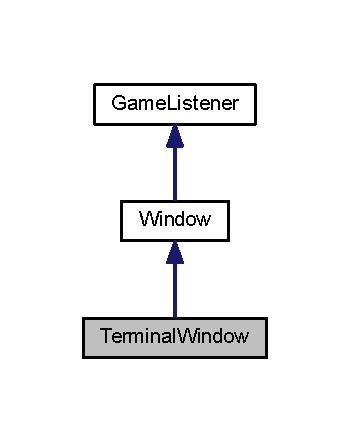
\includegraphics[width=168pt]{class_terminal_window__inherit__graph}
\end{center}
\end{figure}


Collaboration diagram for Terminal\+Window\+:\nopagebreak
\begin{figure}[H]
\begin{center}
\leavevmode
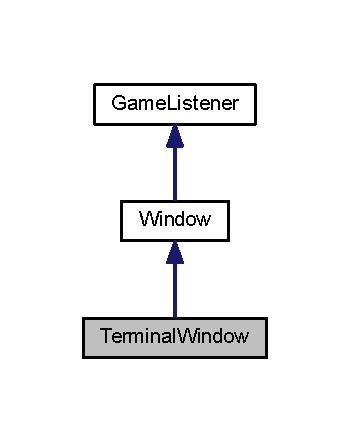
\includegraphics[width=168pt]{class_terminal_window__coll__graph}
\end{center}
\end{figure}
\subsection*{Public Member Functions}
\begin{DoxyCompactItemize}
\item 
\hypertarget{class_terminal_window_a7b89a7a0cfb640d6ae525d953dedce1d}{}\label{class_terminal_window_a7b89a7a0cfb640d6ae525d953dedce1d} 
{\bfseries Terminal\+Window} (int x, int y, int w, int h)
\item 
\hypertarget{class_terminal_window_ab75d0fc5b3ed21c027c5104eb569d347}{}\label{class_terminal_window_ab75d0fc5b3ed21c027c5104eb569d347} 
{\bfseries Terminal\+Window} (const std\+::string \&name, int x, int y, int w, int h)
\item 
\hypertarget{class_terminal_window_a30a31d7c6db112eb5d6e83d0b15f16c5}{}\label{class_terminal_window_a30a31d7c6db112eb5d6e83d0b15f16c5} 
{\bfseries Terminal\+Window} (\hyperlink{class_filesystem}{Filesystem} $\ast$f, const std\+::string \&name, bool movable, int x, int y, int w, int h)
\item 
\hypertarget{class_terminal_window_a263373e2b1075577b559e4b15cae5129}{}\label{class_terminal_window_a263373e2b1075577b559e4b15cae5129} 
void {\bfseries println} (const std\+::string \&s)
\item 
\hypertarget{class_terminal_window_aa73dac9edcb57067e7f662ba9886d16e}{}\label{class_terminal_window_aa73dac9edcb57067e7f662ba9886d16e} 
void {\bfseries print} (const std\+::string \&s)
\item 
\hypertarget{class_terminal_window_a11075e3cd2358dec17179b738d24e744}{}\label{class_terminal_window_a11075e3cd2358dec17179b738d24e744} 
void {\bfseries delayed\+Print} (const std\+::string \&s, int delay)
\item 
\hypertarget{class_terminal_window_ad8c7ad0aa81a42bfc0c65b32d99b37cb}{}\label{class_terminal_window_ad8c7ad0aa81a42bfc0c65b32d99b37cb} 
void {\bfseries draw\+Extra} (\hyperlink{class_graphics}{Graphics} \&g) override
\item 
\hypertarget{class_terminal_window_af82db18ec900835a3489281265bd3601}{}\label{class_terminal_window_af82db18ec900835a3489281265bd3601} 
void {\bfseries update} (float delta) override
\item 
\hypertarget{class_terminal_window_a96697b91e22369a25ccd373c6d576bce}{}\label{class_terminal_window_a96697b91e22369a25ccd373c6d576bce} 
void {\bfseries on\+Input} (const std\+::string \&in) override
\item 
\hypertarget{class_terminal_window_a7c3057b502b117dcfd763e786a482e6b}{}\label{class_terminal_window_a7c3057b502b117dcfd763e786a482e6b} 
void {\bfseries execute\+Command} (const std\+::string \&s)
\item 
\hypertarget{class_terminal_window_a81e9b81579f3fd8dc6c280d6559624de}{}\label{class_terminal_window_a81e9b81579f3fd8dc6c280d6559624de} 
void {\bfseries on\+Special\+Key} (S\+D\+L\+\_\+\+Scancode s) override
\item 
\hypertarget{class_terminal_window_af0ab0a2830652ce7ae40e0ffbc9ee482}{}\label{class_terminal_window_af0ab0a2830652ce7ae40e0ffbc9ee482} 
void {\bfseries on\+Focus} () override
\item 
\hypertarget{class_terminal_window_a7990b694e414bbf6ce3316acb3e827b9}{}\label{class_terminal_window_a7990b694e414bbf6ce3316acb3e827b9} 
void {\bfseries on\+Unfocus} () override
\item 
\hypertarget{class_terminal_window_a85692de7d9dbaeabf1787e30d7747728}{}\label{class_terminal_window_a85692de7d9dbaeabf1787e30d7747728} 
void {\bfseries on\+Filesystem\+Change} (\hyperlink{class_filesystem}{Filesystem} $\ast$f) override
\end{DoxyCompactItemize}
\subsection*{Additional Inherited Members}


The documentation for this class was generated from the following files\+:\begin{DoxyCompactItemize}
\item 
headers/Terminal\+Window.\+h\item 
src/Terminal\+Window.\+cpp\end{DoxyCompactItemize}

\hypertarget{class_window}{}\section{Window Class Reference}
\label{class_window}\index{Window@{Window}}


Inheritance diagram for Window\+:\nopagebreak
\begin{figure}[H]
\begin{center}
\leavevmode
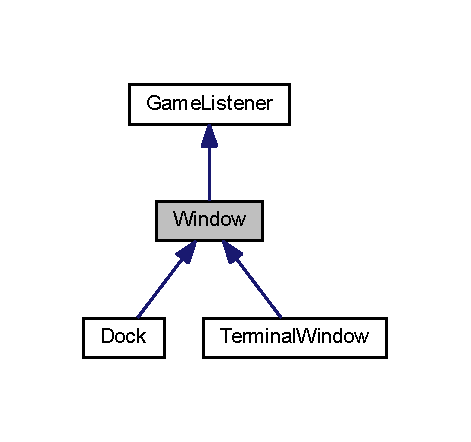
\includegraphics[width=226pt]{class_window__inherit__graph}
\end{center}
\end{figure}


Collaboration diagram for Window\+:\nopagebreak
\begin{figure}[H]
\begin{center}
\leavevmode
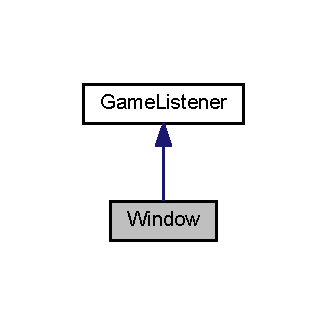
\includegraphics[width=157pt]{class_window__coll__graph}
\end{center}
\end{figure}
\subsection*{Public Member Functions}
\begin{DoxyCompactItemize}
\item 
\hypertarget{class_window_a13073c18448edb5af37659eb910a6457}{}\label{class_window_a13073c18448edb5af37659eb910a6457} 
{\bfseries Window} (const std\+::string \&title, int x, int y, int w, int h)
\item 
\hypertarget{class_window_a00f3bcd540087f25bf85fbc14260c6a6}{}\label{class_window_a00f3bcd540087f25bf85fbc14260c6a6} 
virtual void {\bfseries move} (int x, int y)
\item 
\hypertarget{class_window_a4691b11ae3bf79e96b5c64e4cc1db91e}{}\label{class_window_a4691b11ae3bf79e96b5c64e4cc1db91e} 
virtual void {\bfseries draw} (\hyperlink{class_graphics}{Graphics} \&g)
\item 
\hypertarget{class_window_a00e804d5f11153887fde65f9298c4723}{}\label{class_window_a00e804d5f11153887fde65f9298c4723} 
virtual void {\bfseries draw\+Extra} (\hyperlink{class_graphics}{Graphics} \&g)
\item 
\hypertarget{class_window_addf18acb7913c944b252a9e1d829d870}{}\label{class_window_addf18acb7913c944b252a9e1d829d870} 
virtual void {\bfseries update} (float delta)
\item 
\hypertarget{class_window_ac3a94fd42d4cb51d70f5b20e5c358b8c}{}\label{class_window_ac3a94fd42d4cb51d70f5b20e5c358b8c} 
virtual void {\bfseries on\+Input} (const std\+::string \&input)
\item 
\hypertarget{class_window_ac8219c38f63a27e107e11c0ce996c8ee}{}\label{class_window_ac8219c38f63a27e107e11c0ce996c8ee} 
virtual void {\bfseries on\+Special\+Key} (S\+D\+L\+\_\+\+Scancode key)
\item 
\hypertarget{class_window_a856e913fd554818e67c8bc0734f3b657}{}\label{class_window_a856e913fd554818e67c8bc0734f3b657} 
virtual void {\bfseries on\+Focus} ()
\item 
\hypertarget{class_window_ab849a2c1b4c39b1940c3850d7b0c4dc4}{}\label{class_window_ab849a2c1b4c39b1940c3850d7b0c4dc4} 
virtual void {\bfseries on\+Unfocus} ()
\item 
\hypertarget{class_window_a1284aaa97faa73b4134f7dbf96855cb9}{}\label{class_window_a1284aaa97faa73b4134f7dbf96855cb9} 
virtual void {\bfseries on\+Filesystem\+Change} (\hyperlink{class_filesystem}{Filesystem} $\ast$f)
\item 
\hypertarget{class_window_a5736b4b3555f5a3dd28b6348f7ef4495}{}\label{class_window_a5736b4b3555f5a3dd28b6348f7ef4495} 
void {\bfseries minimize} (bool b)
\item 
\hypertarget{class_window_af602ba77befac67a28be115077bd2879}{}\label{class_window_af602ba77befac67a28be115077bd2879} 
virtual void {\bfseries on\+Mouse} (bool b, int x, int y)
\item 
\hypertarget{class_window_ac3d60de0a45e3ebca44c65176074ebaa}{}\label{class_window_ac3d60de0a45e3ebca44c65176074ebaa} 
void {\bfseries on\+Mouse\+Motion} (S\+D\+L\+\_\+\+Mouse\+Motion\+Event m)
\end{DoxyCompactItemize}
\subsection*{Public Attributes}
\begin{DoxyCompactItemize}
\item 
\hypertarget{class_window_a5d4096105823af83ad842d52f297aa38}{}\label{class_window_a5d4096105823af83ad842d52f297aa38} 
std\+::string {\bfseries \+\_\+title}
\item 
\hypertarget{class_window_af907a6d65dbddffb8e58e162e22472e3}{}\label{class_window_af907a6d65dbddffb8e58e162e22472e3} 
int {\bfseries \+\_\+x}
\item 
\hypertarget{class_window_a40112a204e3a41a989ab7d4d55107390}{}\label{class_window_a40112a204e3a41a989ab7d4d55107390} 
int {\bfseries \+\_\+y}
\item 
\hypertarget{class_window_a7b1f17770125610dd478a0e68072d3da}{}\label{class_window_a7b1f17770125610dd478a0e68072d3da} 
int {\bfseries \+\_\+w}
\item 
\hypertarget{class_window_aab287f182e3d0db85341995ad1375b71}{}\label{class_window_aab287f182e3d0db85341995ad1375b71} 
int {\bfseries \+\_\+h}
\end{DoxyCompactItemize}
\subsection*{Protected Attributes}
\begin{DoxyCompactItemize}
\item 
\hypertarget{class_window_a740438df63489d2c93b3c6eb65da8e94}{}\label{class_window_a740438df63489d2c93b3c6eb65da8e94} 
bool {\bfseries \+\_\+minimized}
\item 
\hypertarget{class_window_a7b3113c737ef37d82ff2d18f3fb82f59}{}\label{class_window_a7b3113c737ef37d82ff2d18f3fb82f59} 
bool {\bfseries \+\_\+moving}
\end{DoxyCompactItemize}


The documentation for this class was generated from the following files\+:\begin{DoxyCompactItemize}
\item 
headers/Window.\+h\item 
src/Window.\+cpp\end{DoxyCompactItemize}

%--- End generated contents ---

% Index
\backmatter
\newpage
\phantomsection
\clearemptydoublepage
\addcontentsline{toc}{chapter}{Index}
\printindex

\end{document}
